\section{Supplementary results}

\subsection{Accuracy by target and scheme}
Table~\ref{tab:accuracy} gives the accuracy for all three targets at each level of novelty, with the settings chosen inside
each split (nested, the estimates of the main text) and with the deployed settings. The 80\% ranges released with the
predictions were set from the held-out residuals of the deployed scheme. On the nested held-out predictions they contain
\CoverSameGenus\% to \CoverNewOrder\% of the measured doubling times at the growth temperature, \CoverRefMin\% to
\CoverRefMax\% of the doubling times at \TRefC\,\textdegree C and \CoverTempMin\% to \CoverTempMax\% of the growth
temperatures, depending on the level, so they can be read as 80\% ranges; the range for the growth temperature is
slightly wide.

\begin{table}[ht]\centering\small
\caption{Accuracy by closest labeled relative, mean of 3 seeds. Error is the typical fold error for doubling times and the mean absolute error in \textdegree C for growth temperature; $\rho$ is the Spearman correlation. Nested: settings chosen inside each split, each training genome entered once per placement rank, as deployed (the estimates quoted in the main text). Fixed, coarsened: the deployed settings, chosen on all rows, with the deployed training scheme. Fixed, single: the deployed settings and each genome entered once.}\label{tab:accuracy}
\begin{tabular}{lcccccccc}
\toprule
& \multicolumn{2}{c}{same genus} & \multicolumn{2}{c}{new genus} & \multicolumn{2}{c}{new family} & \multicolumn{2}{c}{new order} \\
\cmidrule(lr){2-3} \cmidrule(lr){4-5} \cmidrule(lr){6-7} \cmidrule(lr){8-9}
& Error & $\rho$ & Error & $\rho$ & Error & $\rho$ & Error & $\rho$ \\
\midrule
\multicolumn{9}{l}{\textit{Doubling time at the growth temperature}} \\
\quad nested & 1.75 & 0.74 & 1.91 & 0.71 & 2.06 & 0.66 & 2.08 & 0.66 \\
\quad fixed, coarsened & 1.75 & 0.74 & 1.92 & 0.71 & 2.07 & 0.67 & 2.08 & 0.66 \\
\quad fixed, single & 1.82 & 0.74 & 1.96 & 0.71 & 2.07 & 0.67 & 2.08 & 0.67 \\
\multicolumn{9}{l}{\textit{Doubling time at 20 \textdegree C}} \\
\quad nested & 1.73 & 0.84 & 1.81 & 0.83 & 1.91 & 0.81 & 1.93 & 0.81 \\
\quad fixed, coarsened & 1.73 & 0.84 & 1.81 & 0.83 & 1.88 & 0.82 & 1.93 & 0.81 \\
\quad fixed, single & 1.75 & 0.84 & 1.79 & 0.83 & 1.88 & 0.82 & 1.91 & 0.81 \\
\multicolumn{9}{l}{\textit{Growth temperature}} \\
\quad nested & 4.96 & 0.86 & 5.74 & 0.83 & 5.81 & 0.83 & 5.99 & 0.81 \\
\quad fixed, coarsened & 5.13 & 0.85 & 5.77 & 0.83 & 5.87 & 0.82 & 6.07 & 0.81 \\
\quad fixed, single & 5.36 & 0.85 & 5.88 & 0.82 & 5.96 & 0.82 & 6.15 & 0.81 \\
\bottomrule
\end{tabular}
\end{table}


\subsection{Ranges by group and the probability of slow growth}
Table~\ref{tab:ranges} gives the coverage of the 80\% ranges by group of genomes, and Table~\ref{tab:slowprob} the
probability of growing slower than a day (Methods). The released ranges are those by novelty level and domain.

\begin{table}[ht]\centering\small
\caption{Coverage (\%) of the 80\% ranges for the doubling time at the growth temperature, cross-fitted over genera, by group of genomes, for ranges set by novelty level alone and by novelty level and domain (released). Groups by the true doubling time cannot be targeted by any range built from the inputs.}\label{tab:ranges}
\begin{tabular}{llccccc}
\toprule
Held out & Ranges by & All & Bacteria & Archaea & Fast in truth & Slow in truth \\
\midrule
same genus & novelty & 80 & 80 & 79 & 83 & 44 \\
 & novelty, domain & 80 & 80 & 79 & 83 & 45 \\
new genus & novelty & 80 & 80 & 80 & 83 & 36 \\
 & novelty, domain & 79 & 79 & 79 & 83 & 37 \\
new family & novelty & 80 & 79 & 81 & 84 & 29 \\
 & novelty, domain & 80 & 80 & 80 & 84 & 29 \\
new order & novelty & 80 & 82 & 73 & 85 & 26 \\
 & novelty, domain & 79 & 79 & 78 & 83 & 29 \\
\bottomrule
\end{tabular}
\end{table}

\begin{table}[ht]\centering\small
\caption{The probability of a doubling time above 24 h (logistic model on the predicted log doubling time and the domain), cross-fitted over genera, by the closest labeled relative. Calibration error: mean absolute difference between predicted probability and observed share over fifths of the predicted probability.}\label{tab:slowprob}
\begin{tabular}{lcccc}
\toprule
& same genus & new genus & new family & new order \\
\midrule
AUC & 0.84 & 0.83 & 0.79 & 0.81 \\
Brier score & 0.057 & 0.060 & 0.066 & 0.065 \\
Brier score of the base rate & 0.072 & 0.072 & 0.072 & 0.072 \\
calibration error & 0.010 & 0.008 & 0.009 & 0.012 \\
slow among the top fifth & 0.24 & 0.25 & 0.22 & 0.22 \\
slow overall & 0.08 & 0.08 & 0.08 & 0.08 \\
\bottomrule
\end{tabular}
\end{table}


\subsection{Pressure tests}
Table~\ref{tab:pressure} compares the nested model with two baselines scored on the same folds, gives bootstrap intervals,
and reports the shuffled-label control (Methods).

\begin{table}[ht]\centering\small
\caption{Pressure tests of the headline (doubling time at the growth temperature, mean of 3 seeds, the folds of the headline). Intervals: 95\% bootstrap over species groups; for this model, of the typical error and Spearman correlation; for the median of the closest relatives, of the model's error minus the baseline's (negative: the model is better). Shuffled labels: the deployed model trained and scored on labels permuted across genomes.}\label{tab:pressure}
\begin{tabular}{lcccc}
\toprule
& Error ($\times$) & Spearman & AUC, slow & 95\% interval \\
\midrule
\multicolumn{5}{l}{\textit{Same genus}} \\
\quad this model, nested & 1.75 & 0.74 & 0.85 & 1.67--1.86, 0.68--0.78 \\
\quad median of closest relatives & 1.81 & 0.66 & 0.80 & $-$0.21 to +0.05 \\
\quad median training label & 2.72 & $-$0.08 & 0.45 &  \\
\multicolumn{5}{l}{\textit{New genus}} \\
\quad this model, nested & 1.91 & 0.71 & 0.84 & 1.81--2.02, 0.66--0.76 \\
\quad median of closest relatives & 2.12 & 0.57 & 0.79 & $-$0.42 to $-$0.02 \\
\quad median training label & 2.74 & $-$0.07 & 0.47 &  \\
\multicolumn{5}{l}{\textit{New family}} \\
\quad this model, nested & 2.06 & 0.66 & 0.81 & 1.93--2.24, 0.59--0.72 \\
\quad median of closest relatives & 2.59 & 0.40 & 0.72 & $-$0.84 to $-$0.21 \\
\quad median training label & 2.86 & $-$0.20 & 0.43 &  \\
\multicolumn{5}{l}{\textit{New order}} \\
\quad this model, nested & 2.08 & 0.66 & 0.82 & 1.96--2.23, 0.57--0.72 \\
\quad median of closest relatives & 2.45 & 0.41 & 0.72 & $-$0.74 to $-$0.16 \\
\quad median training label & 2.78 & $-$0.18 & 0.40 &  \\
\multicolumn{5}{l}{\textit{Labels shuffled across genomes}} \\
\quad this model, species held out & 2.91 & 0.00 & 0.49 & \\
\quad median training label, species held out & 2.73 & $-$0.03 & 0.50 & \\
\quad this model, order held out & 2.89 & $-$0.04 & 0.47 & \\
\quad median training label, order held out & 2.72 & $-$0.06 & 0.45 & \\
\bottomrule
\end{tabular}
\end{table}


\subsection{Leakage, label and split robustness}
Table~\ref{tab:robust} reports three further checks: the model against the relatives' median over \TenNSeeds seeds instead
of three, the effect of gRodon's released estimate (whose coefficients saw our species) against a refit inside each split,
and the effect of the labels from studies that the study-level check flagged but that we kept.

\begin{table}[ht]\centering\footnotesize\setlength{\tabcolsep}{3pt}
\caption{Robustness checks, deployed settings and each genome once, 10 seeds on the official splits. Errors are typical fold errors of the first and second method (a, b); seeds and genomes: how many favour a; $p$: paired Wilcoxon test over genomes (absolute log errors averaged over seeds). The refit replaces gRodon's released estimate, whose coefficients were fitted on data that include our species, with a regression of the log doubling time on gRodon's codon statistics fitted on the training rows of each split. The flagged-study test removes the labels of the studies flagged by the study-level check but kept, and scores both models on the remaining genomes.}\label{tab:robust}
\begin{tabular}{llcccccccc}
\toprule
Comparison (a vs b) & Held out & Genomes & Error a & Error b & $\rho$ a & $\rho$ b & Seeds & Genomes & $p$ \\
\midrule
model vs relatives' median & species & 741 & 1.822 & 1.793 & 0.74 & 0.67 & 3/10 & 392 & 0.018 \\
without gRodon's estimate vs full & species & 741 & 1.863 & 1.822 & 0.72 & 0.74 & 1/10 & 328 & 0.003 \\
gRodon refitted in each split vs full & species & 741 & 1.851 & 1.822 & 0.73 & 0.74 & 0/10 & 357 & 0.086 \\
without flagged-study labels vs full & species & 716 & 1.790 & 1.807 & 0.75 & 0.74 & 7/10 & 381 & 0.038 \\
model vs relatives' median & genus & 741 & 1.912 & 2.152 & 0.71 & 0.55 & 10/10 & 431 & $<$0.001 \\
model vs relatives' median & family & 741 & 2.025 & 2.597 & 0.68 & 0.40 & 10/10 & 496 & $<$0.001 \\
model vs relatives' median & order & 741 & 2.081 & 2.412 & 0.66 & 0.40 & 10/10 & 444 & $<$0.001 \\
without gRodon's estimate vs full & order & 741 & 2.154 & 2.081 & 0.63 & 0.66 & 0/10 & 303 & $<$0.001 \\
gRodon refitted in each split vs full & order & 741 & 2.104 & 2.081 & 0.64 & 0.66 & 3/10 & 328 & $<$0.001 \\
without flagged-study labels vs full & order & 716 & 2.023 & 2.046 & 0.68 & 0.67 & 8/10 & 392 & 0.003 \\
\bottomrule
\end{tabular}
\end{table}


\subsection{External test}
Table~\ref{tab:external} lists the \ExtN species of the external test with their measured and predicted doubling times and
the source of each value. With orders held out, the comparison with the released tools gives the errors in the main text;
the per-genome predictions are released with the data.

{\footnotesize\setlength{\tabcolsep}{3pt}
\begin{longtable}{llcccccl}
\caption{External test: 48 species whose doubling time comes from the species description and that are in neither the Madin compilation (by NCBI taxonomy identifier) nor our labels, with no GTDB species in training. Measured, predicted and relatives' median doubling times in hours at the growth temperature; $T$: the growth temperature stated with the value (\textdegree C, blank where none was stated); range: whether the measured value lies inside the released 80\% range.}\label{tab:external}\\
\toprule
Species & Closest labeled relative & $T$ & Measured & Predicted & Relatives & Range & Source \\
\midrule
\endfirsthead
\toprule
Species & Closest labeled relative & $T$ & Measured & Predicted & Relatives & Range & Source \\
\midrule
\endhead
\textit{Carboxydothermus islandicus} & same genus &  & 2 & 1.94 & 2 & yes & PMID 21131500 \\
\textit{Carboxydothermus pertinax} & same genus &  & 1.5 & 3.19 & 2 & yes & PMID 21908679 \\
\textit{Hydrogenimonas urashimensis} & same genus &  & 3 & 2.99 & 1.16 & yes & PMID 33340909 \\
\textit{Methanospirillum purgamenti} & same genus & 35 & 10 & 9.78 & 20.7 & yes & PMID 39186748 \\
\textit{Methylacidiphilum kamchatkense} & same genus & 55 & 6.3 & 8.73 & 9.9 & yes & PMID 37755432 \\
\textit{Paracoccus solventivorans} & same genus &  & 12 & 5.21 & 2.1 & yes & PMID 8863446 \\
\textit{Thermocrinis jamiesonii} & same genus &  & 1.3 & 1.5 & 1.18 & yes & PMID 26419502 \\
\textit{Aminomonas paucivorans} & same family, new genus & 35 & 16 & 2.36 & 63.3 & no & PMID 10425753 \\
\textit{Anaerobium acetethylicum} & same family, new genus & 30 & 1 & 0.59 & 4.35 & yes & PMID 26297346 \\
\textit{Anaeromicrobium sediminis} & same family, new genus & 37 & 1.27 & 1.7 & 5.73 & yes & PMID 27974087 \\
\textit{Aureliella helgolandensis} & same family, new genus &  & 41 & 15.2 & 10 & yes & PMID 32219667 \\
\textit{Caloramator quimbayensis} & same family, new genus & 50 & 2 & 2.63 & 0.324 & yes & PMID 22843719 \\
\textit{Methanothermococcus jasoni} & same family, new genus & 73 & 0.533 & 0.688 & 0.917 & yes & PMID 41773501 \\
\textit{Ornatilinea apprima} & same family, new genus &  & 6 & 48.7 & 50 & no & PMID 22328612 \\
\textit{Persephonella hydrogeniphila} & same family, new genus &  & 0.667 & 2.2 & 2.44 & yes & PMID 12807214 \\
\textit{Phorcysia thermohydrogeniphila} & same family, new genus &  & 0.433 & 1.15 & 1.56 & yes & PMID 22140151 \\
\textit{Spiroplasma corruscae} & same family, new genus & 32 & 1.5 & 4.4 & 2.27 & yes & PMID 8863421 \\
\textit{Spiroplasma eriocheiris} & same family, new genus &  & 24 & 5.11 & 2.27 & no & PMID 20418415 \\
\textit{Spiroplasma poulsonii} & same family, new genus & 30 & 15.8 & 9.82 & 2.27 & yes & PMID 10319483 \\
\textit{Spiroplasma syrphidicola} & same family, new genus &  & 1 & 2.55 & 2.27 & yes & PMID 8782692 \\
\textit{Sulfurovum aggregans} & same family, new genus &  & 3.2 & 1.64 & 1.84 & yes & PMID 24966202 \\
\textit{Sulfurovum riftiae} & same family, new genus &  & 3 & 1.61 & 1.84 & yes & PMID 27116914 \\
\textit{Tautonia plasticadhaerens} & same family, new genus &  & 29 & 8.54 & 17.4 & no & PMID 32399714 \\
\textit{Thermocrinis minervae} & same family, new genus & 75 & 4.5 & 1.97 & 1.4 & yes & PMID 19651724 \\
\textit{Varunaivibrio sulfuroxidans} & same family, new genus &  & 8 & 8.56 & 11 & yes & PMID 27298285 \\
\textit{Deferribacter autotrophicus} & same order, new family &  & 1 & 5.54 & 8.42 & no & PMID 19502344 \\
\textit{Deferribacter desulfuricans} & same order, new family &  & 0.667 & 6.19 & 8.42 & no & PMID 12807210 \\
\textit{Defluviitalea raffinosedens} & same order, new family & 50 & 1.2 & 3 & 4.35 & yes & PMC5817277 \\
\textit{Desulfovulcanus ferrireducens} & same order, new family & 65 & 7.1 & 11.1 & 16.7 & yes & PMID 35190935 \\
\textit{Fervidicoccus fontis} & same order, new family & 67.5 & 6.1 & 3.2 & 3.71 & yes & PMID 19837732 \\
\textit{Lentimicrobium saccharophilum} & same order, new family &  & 24 & 11.8 & 1.47 & yes & PMID 27098854 \\
\textit{Spiroplasma platyhelix} & same order, new family & 30 & 6.4 & 2.36 & 2.72 & yes & PMID 9226909 \\
\textit{Sporanaerobium hydrogeniformans} & same order, new family &  & 5 & 0.87 & 4.35 & no & PMID 37572166 \\
\textit{Sulfurimonas hongkongensis} & same order, new family & 30 & 6.1 & 1.73 & 1.22 & yes & PMC4149026 \\
\textit{Aggregatilinea lenta} & new order &  & 456 & 11.2 & 50 & no & PMID 30775966 \\
\textit{Anoxybacter fermentans} & new order & 60 & 0.45 & 1.37 & 3.5 & yes & PMID 25505345 \\
\textit{Atrimonas thermophila} & new order & 72.5 & 11.4 & 2.2 & 2.1 & no & PMID 38776610 \\
\textit{Brockia lithotrophica} & new order & 62.5 & 6 & 1.3 & 0.5 & no & PMID 22493174 \\
\textit{Caldanaerovirga acetigignens} & new order &  & 3.4 & 2.73 & 1.25 & yes & PMID 19625440 \\
\textit{Calderihabitans maritimus} & new order & 65 & 3.7 & 3.44 & 1.25 & yes & PMID 23606483 \\
\textit{Carboxydocella thermautotrophica} & new order &  & 1.1 & 1.54 & 1.25 & yes & PMID 12508854 \\
\textit{Deferrisoma palaeochoriense} & new order &  & 2.5 & 2.77 & 12.4 & yes & PMID 26610851 \\
\textit{Desulfobacca acetoxidans} & new order & 37 & 48 & 10.1 & 12.4 & no & PMID 10319454 \\
\textit{Desulfocarbo indianensis} & new order & 30 & 64.8 & 13.4 & 12.4 & no & PMID 24876241 \\
\textit{Mariprofundus micogutta} & new order & 25 & 24 & 2.48 & 1.73 & no & PMID 27766355 \\
\textit{Phosphitispora fastidiosa} & new order & 30 & 72 & 7.39 & 1.25 & no & PMID 34878375 \\
\textit{Stratiformator vulcanicus} & new order &  & 102 & 20.5 & 13.2 & no & PMID 37584762 \\
\textit{Thermincola carboxydiphila} & new order &  & 1.3 & 6 & 1.25 & no & PMID 16166711 \\
\bottomrule
\end{longtable}}


\subsection{Comparison with released gRodon and Phydon}
\begin{table}[ht]\centering\small
\caption{Comparison with the released gRodon and Phydon on the same genomes and folds (species held out, mean of 3 seeds), with our model built inside each split as deployed.}\label{tab:released}
\begin{tabular}{lcccc}
\toprule
& Genomes & Typical error ($\times$) & Spearman & AUC, slow \\
\midrule
\multicolumn{5}{l}{\textit{All genomes}} \\
\quad This model & 680 & 1.76 & 0.72 & 0.85 \\
\quad This model, given the temperature & 680 & 1.70 & 0.76 & 0.87 \\
\quad gRodon & 680 & 2.40 & 0.52 & 0.75 \\
\quad gRodon, given the temperature & 680 & 1.92 & 0.73 & 0.84 \\
\quad Phydon, given the temperature & 665 & 1.85 & 0.70 & 0.81 \\
\multicolumn{5}{l}{\textit{Phydon found the species on its tree}} \\
\quad This model & 665 & 1.76 & 0.71 & 0.85 \\
\quad This model, given the temperature & 665 & 1.70 & 0.76 & 0.87 \\
\quad gRodon & 665 & 2.41 & 0.52 & 0.75 \\
\quad gRodon, given the temperature & 665 & 1.92 & 0.73 & 0.84 \\
\quad Phydon, given the temperature & 665 & 1.85 & 0.70 & 0.81 \\
\bottomrule
\end{tabular}
\end{table}


\begin{figure}[ht]
\centering
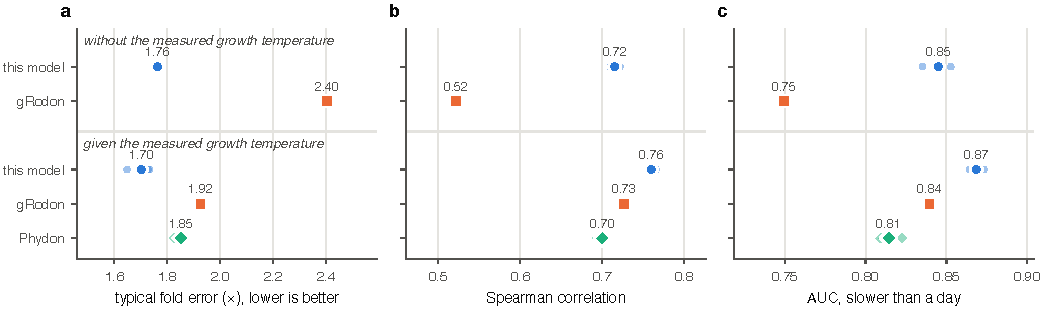
\includegraphics[width=\textwidth]{fig3_released_tools}
\caption{The released gRodon and Phydon against this model on the same \RelN genomes, genes and species-held-out folds
(\RelNSeeds seeds; small marks are seeds, large marks their mean). Both released tools take the measured growth
temperature, which an uncultured genome does not come with; this model is shown without it and with it added as an input.
(a) Typical fold error. (b) Spearman correlation. (c) Area under the curve for a doubling time above one day.}
\label{fig:released}
\end{figure}

\subsection{Ablations at each level}
Table~\ref{tab:ablationsfull} gives the absolute values behind the ablation table of the main text, and the family level,
which the main text leaves out.

\begin{table}[ht]\centering\small
\caption{Every ablation at each held-out level, mean (standard deviation) over 10 seeds, with the deployed settings and each genome entered once. The ablation table of the main text gives the paired changes at the species and order levels.}\label{tab:ablationsfull}
\begin{tabular}{lccc}
\toprule
& Typical error ($\times$) & Spearman & AUC, slow \\
\midrule
\multicolumn{4}{l}{\textit{Species held out}} \\
\quad final model & 1.819 (0.013) & 0.740 (0.005) & 0.838 (0.005) \\
\quad without gRodon statistics & 1.929 (0.024) & 0.697 (0.005) & 0.828 (0.005) \\
\quad without lifestyle genes & 1.824 (0.016) & 0.738 (0.005) & 0.838 (0.005) \\
\quad without any gene features & 2.092 (0.029) & 0.662 (0.004) & 0.806 (0.007) \\
\quad without 16S & 1.817 (0.018) & 0.742 (0.006) & 0.839 (0.005) \\
\quad without GTDB phylogeny & 1.844 (0.029) & 0.732 (0.005) & 0.840 (0.005) \\
\quad without the added species & 1.859 (0.031) & 0.732 (0.007) & 0.836 (0.005) \\
\quad with energy-metabolism genes & 1.820 (0.014) & 0.740 (0.005) & 0.839 (0.005) \\
\quad with predicted growth temperature & 1.804 (0.026) & 0.739 (0.005) & 0.839 (0.005) \\
\addlinespace
\multicolumn{4}{l}{\textit{Family held out}} \\
\quad final model & 2.049 (0.035) & 0.675 (0.010) & 0.808 (0.006) \\
\quad without gRodon statistics & 2.269 (0.066) & 0.600 (0.016) & 0.770 (0.013) \\
\quad without lifestyle genes & 2.047 (0.038) & 0.673 (0.011) & 0.808 (0.007) \\
\quad without any gene features & 2.515 (0.075) & 0.510 (0.024) & 0.741 (0.018) \\
\quad without 16S & 2.029 (0.021) & 0.679 (0.008) & 0.802 (0.008) \\
\quad without GTDB phylogeny & 2.038 (0.042) & 0.673 (0.011) & 0.812 (0.007) \\
\quad without the added species & 2.080 (0.049) & 0.667 (0.008) & 0.807 (0.007) \\
\quad with energy-metabolism genes & 2.055 (0.033) & 0.672 (0.009) & 0.809 (0.005) \\
\quad with predicted growth temperature & 2.047 (0.046) & 0.675 (0.010) & 0.810 (0.006) \\
\addlinespace
\multicolumn{4}{l}{\textit{Order held out}} \\
\quad final model & 2.093 (0.028) & 0.654 (0.010) & 0.803 (0.009) \\
\quad without gRodon statistics & 2.388 (0.051) & 0.574 (0.014) & 0.759 (0.012) \\
\quad without lifestyle genes & 2.074 (0.032) & 0.660 (0.009) & 0.805 (0.008) \\
\quad without any gene features & 2.644 (0.049) & 0.460 (0.017) & 0.727 (0.015) \\
\quad without 16S & 2.093 (0.032) & 0.654 (0.012) & 0.793 (0.010) \\
\quad without GTDB phylogeny & 2.070 (0.026) & 0.657 (0.008) & 0.809 (0.009) \\
\quad without the added species & 2.133 (0.025) & 0.650 (0.012) & 0.797 (0.008) \\
\quad with energy-metabolism genes & 2.107 (0.036) & 0.654 (0.010) & 0.802 (0.008) \\
\quad with predicted growth temperature & 2.078 (0.028) & 0.659 (0.012) & 0.805 (0.010) \\
\bottomrule
\end{tabular}
\end{table}


\subsection{A learned-representation baseline}
Table~\ref{tab:esm} compares protein language-model embeddings with the genome features on the folds of the headline
(Methods of the main text).

\begin{table}[ht]\centering\small\setlength{\tabcolsep}{4pt}
\caption{A learned-representation baseline: ESM-2 (35M) protein embeddings of 742 genomes (mean of all ribosomal proteins and of 100 other proteins per genome) against the genome features, on the folds of the headline, deployed settings, each genome once, mean of 3 seeds. Error: typical fold error of the doubling time at the growth temperature; $\rho$: Spearman correlation.}\label{tab:esm}
\begin{tabular}{lcccccccc}
\toprule
& \multicolumn{2}{c}{same genus} & \multicolumn{2}{c}{new genus} & \multicolumn{2}{c}{new family} & \multicolumn{2}{c}{new order} \\
\cmidrule(lr){2-3} \cmidrule(lr){4-5} \cmidrule(lr){6-7} \cmidrule(lr){8-9}
& Error & $\rho$ & Error & $\rho$ & Error & $\rho$ & Error & $\rho$ \\
\midrule
genome features & 1.82 & 0.74 & 1.96 & 0.71 & 2.07 & 0.67 & 2.08 & 0.67 \\
ESM-2, ridge probe & 1.86 & 0.75 & 1.90 & 0.73 & 2.00 & 0.69 & 2.02 & 0.68 \\
ESM-2, trees on 64 PCs & 2.03 & 0.71 & 2.11 & 0.67 & 2.19 & 0.62 & 2.23 & 0.61 \\
genome features + 32 ESM-2 PCs & 1.78 & 0.76 & 1.91 & 0.74 & 2.03 & 0.70 & 2.05 & 0.70 \\
\bottomrule
\end{tabular}
\end{table}


\subsection{Species from other sources}
As a check that does not depend on how the folds are drawn, the final model was trained on gRodon's growth table alone and
tested on every labeled species of the other sources whose species group is not in that table (Table~\ref{tab:independent}).
The typical error over the \IndepN bacterial species is \IndepErr-fold. The archaeal rows show what happens with no archaea
in training and are not a fair test of the deployed model, which is trained on archaea.

\begin{table}[ht]\centering\small
\caption{Species that are not in gRodon's growth table, predicted by the final model trained on that table alone (294 genomes, no archaea), averaged over five seeds. Error is the typical fold error; $\rho$ the Spearman correlation. The training set is less than half of the full one, so these errors are higher than those of the deployed model; the test shows how the model carries to species from other sources.}\label{tab:independent}
\begin{tabular}{lccccc}
\toprule
& & \multicolumn{2}{c}{At the growth temperature} & \multicolumn{2}{c}{At 20 \textdegree C} \\
\cmidrule(lr){3-4} \cmidrule(lr){5-6}
& Species & Error & $\rho$ & Error & $\rho$ \\
\midrule
\multicolumn{6}{l}{\textit{Bacteria, by closest relative in gRodon's growth table}} \\
\quad same genus & 44 & 1.85 & 0.31 & 1.58 & 0.81 \\
\quad same family, new genus & 76 & 1.82 & 0.66 & 1.91 & 0.75 \\
\quad same order, new family & 68 & 1.91 & 0.51 & 1.78 & 0.83 \\
\quad new order & 106 & 2.65 & 0.39 & 2.09 & 0.63 \\
\quad all bacteria & 294 & 2.09 & 0.61 & 1.87 & 0.78 \\
Archaea (none in training) & 150 & 2.46 & 0.57 & 2.54 & 0.43 \\
\bottomrule
\end{tabular}
\end{table}


\subsection{Metagenome-assembled genomes by species}
\begin{longtable}{p{6.2cm}cccc}
\caption{Doubling time at the growth temperature predicted from metagenome-assembled genomes (MAGs, median over the species' MAGs) and from the isolate genome, with the species held out of training, for the 47 species with a measured value and at least one GEM genome; 717 MAGs in all. Both predictions use the model without 16S, which every MAG can be given.}\label{tab:mags}\\
\toprule
Species & MAGs & Measured (h) & Isolate (h) & MAGs (h) \\
\midrule
\endfirsthead
\caption[]{(continued)}\\
\toprule
Species & MAGs & Measured (h) & Isolate (h) & MAGs (h) \\
\midrule
\endhead
\textit{Acinetobacter baumannii} & 7 & 0.73 & 1.22 & 1.17 \\
\textit{Aeromonas hydrophila} & 1 & 0.33 & 0.67 & 0.78 \\
\textit{Allisonella histaminiformans} & 1 & 1.83 & 0.70 & 0.96 \\
\textit{Bacillus licheniformis} & 1 & 0.58 & 0.70 & 1.10 \\
\textit{Bacillus subtilis} & 4 & 0.24 & 0.68 & 1.02 \\
\textit{Bacteroides fragilis} & 19 & 0.44 & 1.97 & 1.53 \\
\textit{Bacteroides thetaiotaomicron} & 11 & 1.47 & 2.94 & 1.32 \\
\textit{Bifidobacterium longum} & 59 & 1.51 & 1.80 & 1.94 \\
\textit{Caldicellulosiruptor obsidiansis} & 1 & 0.92 & 2.57 & 3.34 \\
\textit{Caldicellulosiruptor owensensis} & 2 & 5.41 & 2.00 & 1.93 \\
\textit{Caldilinea aerophila} & 2 & 5.00 & 14.24 & 13.81 \\
\textit{Chloroflexus aurantiacus} & 3 & 2.31 & 12.19 & 12.03 \\
\textit{Corynebacterium pseudodiphtheriticum} & 1 & 0.62 & 2.80 & 2.73 \\
\textit{Cronobacter sakazakii} & 1 & 0.23 & 0.39 & 0.51 \\
\textit{Cutibacterium acnes} & 127 & 5.10 & 2.82 & 2.81 \\
\textit{Dehalococcoides mccartyi\_B} & 2 & 19.20 & 10.16 & 9.30 \\
\textit{Dictyoglomus thermophilum} & 3 & 2.47 & 1.51 & 1.44 \\
\textit{Enterococcus faecalis} & 50 & 0.38 & 1.13 & 0.71 \\
\textit{Escherichia coli} & 178 & 0.18 & 0.64 & 0.64 \\
\textit{Fusobacterium nucleatum} & 2 & 0.47 & 0.86 & 0.93 \\
\textit{Isosphaera pallida} & 1 & 17.35 & 11.71 & 12.01 \\
\textit{Klebsiella pneumoniae} & 29 & 0.34 & 0.39 & 0.40 \\
\textit{Lactobacillus acidophilus} & 1 & 1.10 & 0.67 & 0.75 \\
\textit{Lactococcus lactis} & 14 & 0.39 & 0.50 & 0.67 \\
\textit{Leifsonia xyli\_A} & 1 & 5.50 & 2.28 & 1.39 \\
\textit{Meiothermus ruber} & 1 & 1.67 & 2.07 & 2.01 \\
\textit{Mesotoga prima} & 3 & 16.50 & 3.45 & 4.17 \\
\textit{Nitrosomonas europaea} & 5 & 5.50 & 6.16 & 6.81 \\
\textit{Persephonella marina} & 7 & 3.35 & 1.61 & 1.51 \\
\textit{Porphyromonas gingivalis} & 11 & 2.56 & 6.57 & 6.34 \\
\textit{Pseudomonas aeruginosa} & 5 & 0.33 & 0.52 & 0.68 \\
\textit{Psychrobacter cryohalolentis} & 2 & 2.62 & 2.23 & 2.22 \\
\textit{Rhodopirellula baltica} & 1 & 10.00 & 12.71 & 12.29 \\
\textit{Sinorhizobium meliloti} & 1 & 1.50 & 2.08 & 1.47 \\
\textit{Staphylococcus aureus} & 1 & 0.45 & 0.46 & 0.62 \\
\textit{Staphylococcus epidermidis} & 22 & 0.33 & 0.54 & 0.65 \\
\textit{Streptococcus mutans} & 2 & 1.10 & 0.79 & 0.79 \\
\textit{Streptococcus thermophilus} & 9 & 0.29 & 0.43 & 0.47 \\
\textit{Syntrophobacter fumaroxidans} & 1 & 98.00 & 7.46 & 7.72 \\
\textit{Syntrophus aciditrophicus} & 1 & 27.00 & 3.65 & 3.68 \\
\textit{Thermobaculum terrenum} & 6 & 4.09 & 3.78 & 3.36 \\
\textit{Thermodesulfobacterium commune} & 1 & 2.31 & 1.98 & 1.77 \\
\textit{Thermus aquaticus} & 4 & 0.69 & 0.76 & 0.80 \\
\textit{Thermus brockianus} & 1 & 1.07 & 0.84 & 0.85 \\
\textit{Thermus thermophilus} & 110 & 0.29 & 0.93 & 0.90 \\
\textit{Vibrio alginolyticus} & 1 & 0.25 & 0.46 & 0.46 \\
\textit{Vibrio cholerae} & 1 & 0.35 & 0.43 & 0.47 \\
\bottomrule
\end{longtable}


\subsection{The low-energy test, every input}
Table~\ref{tab:pgls} gives every input of the low-energy test with the three checks described in the Methods. No input that
describes how an organism makes energy reaches an adjusted $p<0.05$ in the main analysis or in any of these three checks. With $\lambda$
fixed at 1, complex I and the number of terminal oxidases go with faster growth; with only the groups placed at their own
GTDB species, catalase does. Regulator density goes with faster growth in the main analysis and in two of the three checks,
but not with $\lambda$ fixed at 1.

{\small\setlength{\tabcolsep}{3pt}
\begin{longtable}{p{4.6cm}rrlrrrrr}
\caption{The low-energy test, every input, 592 species groups. Effects are fold changes in doubling time for carrying the gene, per standard deviation of a count or density, or per doubling of genome size, with growth temperature and domain as covariates. With: groups carrying the gene (presence inputs). Across: without control for relatedness. PGLS: phylogenetic generalized least squares with Pagel's $\lambda$ estimated; $p_{\mathrm{adj}}$ is Benjamini-Hochberg adjusted over the inputs. Families: of the families with both carriers and non-carriers, those in which the median carrier is slower. The last three columns give the adjusted PGLS $p$ with $\lambda$ fixed at 1, with only the groups placed at their own GTDB species, and without the eight literature strains.}\label{tab:pgls}\\
\toprule
Input & With & Across & PGLS (95\% CI) & $p_{\mathrm{adj}}$ & Families & $\lambda=1$ & Own sp. & No lit. \\
\midrule
\endfirsthead
\caption[]{(continued)}\\
\toprule
Input & With & Across & PGLS (95\% CI) & $p_{\mathrm{adj}}$ & Families & $\lambda=1$ & Own sp. & No lit. \\
\midrule
\endhead
aerobic respiration (terminal oxidase) & 393 & 1.14 & 1.01 (0.70--1.45) & 0.992 & 4/8 & 0.601 & 0.904 & 0.993 \\
complex I & 502 & 1.58 & 0.97 (0.72--1.31) & 0.992 & 6/18 & $<$0.001 & 0.886 & 0.993 \\
methanogenesis & 39 & 0.74 & 0.75 (0.27--2.06) & 0.913 & -- & 0.962 & 0.846 & 0.971 \\
sulfate reduction & 24 & 2.84 & 1.33 (0.64--2.78) & 0.852 & 0/2 & 0.962 & 0.846 & 0.754 \\
nitrogen fixation & 128 & 1.52 & 1.18 (0.93--1.50) & 0.595 & 13/26 & 0.385 & 0.846 & 0.435 \\
RuBisCO (carbon fixation) & 172 & 1.21 & 1.15 (0.90--1.46) & 0.700 & 12/26 & 0.332 & 0.846 & 0.697 \\
ammonia or methane oxidation & 7 & 3.76 & 1.49 (0.47--4.77) & 0.901 & -- & 0.962 & 0.846 & 0.993 \\
phototrophy & 31 & 2.51 & 0.92 (0.52--1.65) & 0.992 & 3/6 & 0.962 & 0.904 & 0.993 \\
flagellar motility & 320 & 0.90 & 1.07 (0.80--1.43) & 0.913 & 4/17 & 0.962 & 0.904 & 0.971 \\
catalase & 184 & 0.48 & 0.74 (0.59--0.92) & 0.094 & 16/37 & 0.601 & 0.038 & 0.074 \\
nitrate respiration & 135 & 0.51 & 0.94 (0.72--1.21) & 0.913 & 10/23 & 0.962 & 0.846 & 0.971 \\
denitrification (NosZ) & 63 & 0.95 & 1.04 (0.79--1.38) & 0.992 & 10/24 & 0.962 & 0.886 & 0.971 \\
DMSO/TMAO respiration & 62 & 0.88 & 0.99 (0.73--1.34) & 0.992 & 4/13 & 0.339 & 0.904 & 0.993 \\
fumarate respiration (E. coli type) & 46 & 0.56 & 0.88 (0.55--1.40) & 0.913 & 4/7 & 0.810 & 0.904 & 0.971 \\
metal reduction outside the cell & 16 & 0.47 & 0.64 (0.39--1.06) & 0.393 & 3/8 & 0.339 & 0.505 & 0.435 \\
Wood-Ljungdahl pathway & 66 & 1.29 & 1.19 (0.83--1.72) & 0.763 & 3/9 & 0.962 & 0.886 & 0.697 \\
F-type ATP synthase & 442 & 0.68 & 0.62 (0.39--0.99) & 0.340 & 1/7 & 0.601 & 0.251 & 0.321 \\
V/A-type ATP synthase & 203 & 1.17 & 1.21 (0.92--1.60) & 0.595 & 9/18 & 0.719 & 0.792 & 0.511 \\
Na$^+$-NQR & 67 & 0.42 & 0.76 (0.51--1.15) & 0.595 & 5/9 & 0.859 & 0.792 & 0.624 \\
Rnf complex & 241 & 0.76 & 0.96 (0.77--1.18) & 0.943 & 20/34 & 0.589 & 0.904 & 0.993 \\
Na$^+$-pumping decarboxylase & 171 & 1.03 & 1.15 (0.89--1.48) & 0.713 & 9/17 & 0.339 & 0.846 & 0.697 \\
fermentation only & 122 & 1.04 & 0.98 (0.68--1.39) & 0.992 & 7/11 & 0.962 & 0.846 & 0.993 \\
transporter density (per SD) & -- & 0.83 & 0.88 (0.77--1.00) & 0.340 & -- & 0.478 & 0.085 & 0.435 \\
regulator density (per SD) & -- & 0.78 & 0.80 (0.70--0.92) & 0.042 & -- & 0.408 & 0.018 & 0.049 \\
number of terminal oxidases (per SD) & -- & 0.93 & 0.92 (0.81--1.05) & 0.595 & -- & 0.022 & 0.846 & 0.435 \\
number of hydrogenases (per SD) & -- & 1.20 & 1.13 (1.00--1.27) & 0.340 & -- & 0.962 & 0.792 & 0.321 \\
number of electron acceptor classes (per SD) & -- & 0.92 & 0.99 (0.87--1.13) & 0.992 & -- & 0.601 & 0.904 & 0.993 \\
number of sodium pumps (per SD) & -- & 0.87 & 1.00 (0.88--1.13) & 0.992 & -- & 0.962 & 0.904 & 0.993 \\
genome size (per doubling) & -- & 0.90 & 0.91 (0.75--1.12) & 0.814 & -- & 0.332 & 0.846 & 0.697 \\
\bottomrule
\end{longtable}}

